\documentclass{article} 

\usepackage{amsmath}
\usepackage{mathtools}
\usepackage{amssymb}
\usepackage{xfrac}
\usepackage[margin=1.00in]{geometry}
\usepackage{tabto}
\usepackage{tikz}
\usepackage{pgfplots}


\pgfplotsset{compat = newest}

\title{Testing for plots and whatnot}
\author{Lucas Johnston and Brendan }
\date{\today}

\begin{document}

    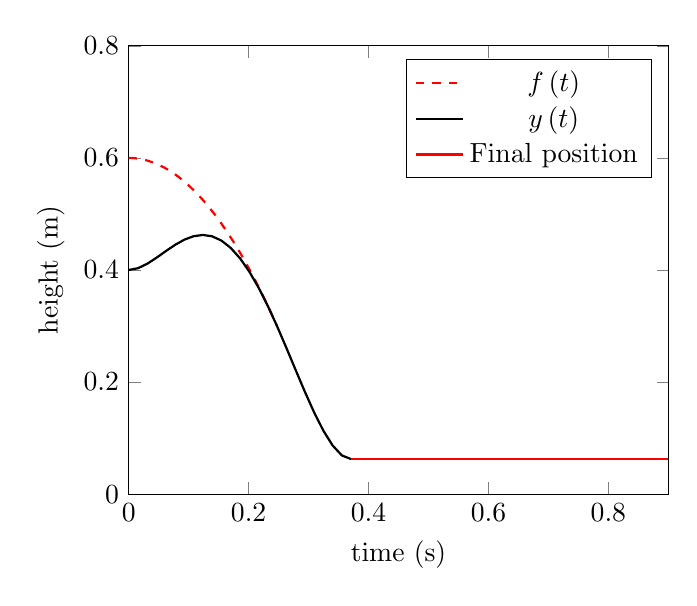
\begin{tikzpicture}
        \begin{axis}[
                xmin = 0,
                xmax = 0.9,
                ymin = 0,
                ymax = 0.8,
                xlabel = time (s),
                ylabel = height (m),
                legend pos=north east, 
                ]
            \addplot[domain = 0:0.247298674822, thick, dashed, red]{0.6-0.5*9.81*x^2};
            \addplot[domain = 0:0.37095212, thick]{160.3981*x^4-105.7772*x^3+14.7141*x^2+0.4};
            \addplot[domain = 0.37095212:0.9, red, thick]{0.0625198478831};
            \legend{$f\left(t\right)$, $y\left(t\right)$, Final position};
        \end{axis}
    \end{tikzpicture}   
\end{document}


 
% \documentclass[pdf-a,balance,colorlinks,upint,subscriptcorrection,varvw,mathalfa=cal=boondoxo, spanish,french,vietnamese,russian,greek]{asmeconf}
% \special{papersize=8.5in,11in}
% 
% \usepackage{amsmath}
% \usepackage{mathtools}
% \usepackage{amssymb}
% \usepackage{xfrac}
% \usepackage[margin=1.00in]{geometry}
% \usepackage{tabto}
% \usepackage{tikz}
% 
% 
% %%%%%  pdf metadata  %%%%%%%%%%%%%%%%%%%%%%%%%%%%%%%%%%%%%%%%%%%%%%%%%%%%%%%%%%%%%%%%%%%%%%%%%%%%%%%%%%
% 
% %%%%%%%%%%%%%%%%%%%%%%%%%%%%%%%%%%%%%%%%%%%%%%%%%%%%%%%%%%%%%%%%%%%%%%%%%%%%%%%%%%%%%%%%%%%%%%%%%%%%%%%
% 
% \begin{document}
% 
% % Change these fields to the right content for your conference.
% % You can comment these out if for some reason you don't want a header.
% % Use title case (first letters capitalized), not all capitals
% 
% \ConfName{Proceedings of the ASME 2024\linebreak International Mechanical Engineering Congress and Exposition}
% \ConfAcronym{IMECE2024}
% \ConfDate{November 17--21, 2024} % update 
% \ConfCity{Portland, OR} % update 
% 
% % Units of measure (e.g., cm) and other specialty lowercase terms in the title should be 
% %   enclosed in \NoCaseChange{...} to maintain lower case type
% %   LaTeX will automatically set the rest of the title in all capital letters.
% 
%     \title{Robot Arm Project}
%     \SetAuthors{Lucas Johnston\affil{1}, Brendan Moskalik\affil{1}}
% 	\SetAffiliation{1}{Gonzaga University, Spokane, WA}
% 
% 
% \maketitle
% 
% 
% %%%%%  End of fields to be completed. Now write your paper. %%%%%%%%%%%%%%%%%%%%%%%%%%%%%%%%%%%%%%%%%%%
% 
% 
% %%%%%  ABSTRACT  %%%%%%%%%%%%%%%%%%%%%%%%%%%%%%%%%%%%%%%%%%%%%%%%%%%
% %%
% %% Abstract should be 200 words or less
% \begin{abstract}
% 
% This paper is an example of and a  {\upshape\LaTeX} template for typesetting ASME conference papers using the {\upshape\texttt{asmeconf}} class. This  {\upshape\LaTeX} template follows ASME guidelines for margins, fonts, headings, captions, and reference formats as of 2024. The class is intended to be used with the {\upshape\texttt{asmeconf.bst} \hologo{BibTeX}} style for reference formatting, which is part of this distribution. The template produces pdfs that contain hyperlinks, bookmarks, and metadata; and references can include the DOI and URL fields. Links may be colored, for online use, or black, for publication. The class enables inline author names, following ASME's current style, but can also produce the traditional grid style. Options include line numbering, final column balancing, various math options, government copyright, and archivability (PDF/A). In addition, section headers may contain mathematics, references, citations, and footnotes. The class is compatible with {\upshape\hologo{pdfLaTeX}} or {\upshape\hologo{LuaLaTeX}}.
% \end{abstract}
% 
% %%%%%%%%%%%%%%%%%%%%%%%%%%%%%%%%%%%%%%%%%%%%%%%%%%%%%%%%%%%
% 
% 
% \end{document}
% 
